%%%%%%%%%%%%%%%%%%%%%%%%%%%%%%%%%%%%%%%%%%%%%%%%%%%%%%%%%%%%%%%%%%%%%%%%%%%%%%%%
\chapter{РАЗРАБОТКА МОДУЛЯ АВТОМАТИЧЕСКОГО ИЗВЛЕЧЕНИЯ КОНТРАКТОВ ДЛЯ СИСТЕМЫ СТАТИЧЕСКОГО АНАЛИЗА BOREALIS}
\label{chapter:developing}
%%%%%%%%%%%%%%%%%%%%%%%%%%%%%%%%%%%%%%%%%%%%%%%%%%%%%%%%%%%%%%%%%%%%%%%%%%%%%%%%
В данном разделе описываются основные этапы разработки модуля автоматического извлечения контрактов для системы Borealis, который реализует описанную ранее технологию.

%%%%%%%%%%%%%%%%%%%%%%%%%%%%%%%%%%%%%%%%%%%%%%%%%%%%%%%%%%%%%%%%%%%%%%%%%%%%%%%%
\section{Архитектура прототипа}
%%%%%%%%%%%%%%%%%%%%%%%%%%%%%%%%%%%%%%%%%%%%%%%%%%%%%%%%%%%%%%%%%%%%%%%%%%%%%%%%
Под прототипом понимается программный модуль, реализующий предложенную методику автоматического извлечения контрактов. Процесс разработки можно разделить на две части: разработка модуля для системы Borealis и разработка библиотеки для работы со встраиваемой базой данных LevelDB\cite{leveldb}.

Структура каталогов модуля для системы Borealis приведена ниже (см. рисунок \ref{image:borealisStructure}).
\begin{figure}[h!]
\center{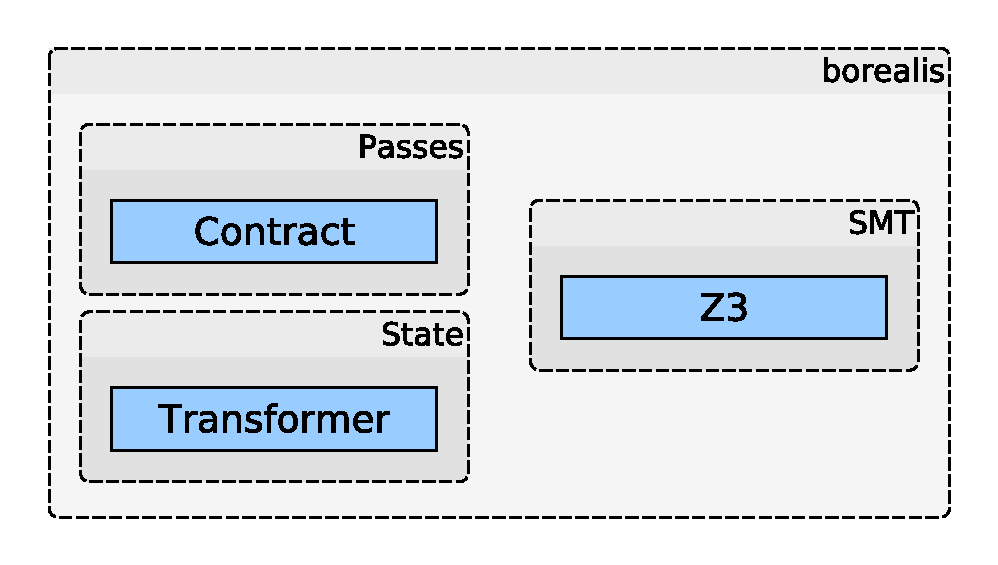
\includegraphics[width=0.75\linewidth]{borealisStructure}}
\caption{Структура каталогов модуля для системы Borealis}
\label{image:borealisStructure}
\end{figure}

Данный модуль реализует предложенную ранее технологию автоматического извлечения контрактов. То есть, он реализует следующие функции: анализ исходного кода и извлечение предварительного множества предикатов, работа с БД для записи/чтения результатов анализа, формирование контрактов для функции и добавление обнаруженных контрактов в систему для выполнения статического анализа.

Структура каталогов библиотеки для работы с LevelDB приведена ниже (см. рисунок \ref{image:leveldbStructure}).
\begin{figure}[h!]
\center{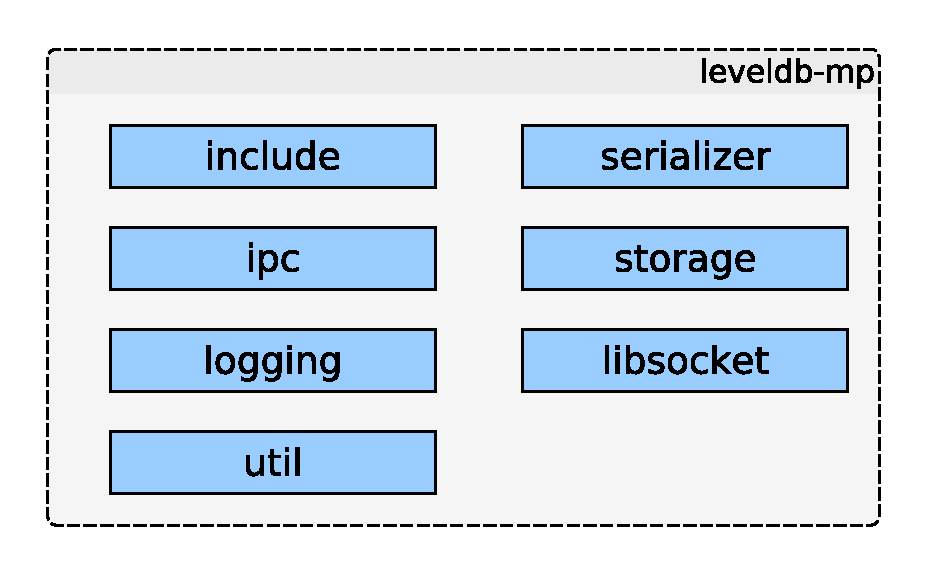
\includegraphics[width=0.75\linewidth]{leveldbStructure}}
\caption{Структура каталогов библиотеки для работы с LevelDB}
\label{image:leveldbStructure}
\end{figure}

В данном проекте реализуются два подпроекта: сервер для непосредственной работы с БД и клиент для подключения к этому серверу. БД используется для хранения результатов анализа.

Рассмотрим реализацию прототипа более подробно.

%%%%%%%%%%%%%%%%%%%%%%%%%%%%%%%%%%%%%%%%%%%%%%%%%%%%%%%%%%%%%%%%%%%%%%%%%%%%%%%%
\section{Разработка библиотеки для взаимодействия с БД}
%%%%%%%%%%%%%%%%%%%%%%%%%%%%%%%%%%%%%%%%%%%%%%%%%%%%%%%%%%%%%%%%%%%%%%%%%%%%%%%%
LevelDB --- встраиваемая база данных, организованная как хранилище пар ключ-значение. Данное хранилище имеет ряд положительных качеств:
\begin{itemize}
\item БД является встраиваемой, то есть она не требует поддержки сервера;
\item БД достаточно проста. Она не поддерживает SQL и работа с ней происходит с помощью простых запросов put/get;
\item возможность итерирования по данным;
\item БД обладает достаточно высокой производительностью\footnote{http://leveldb.googlecode.com/svn/trunk/doc/benchmark.html};
\end{itemize}

LevelDB имеет одну отрицательную характеристику: она не поддерживает одновременное подключение нескольких потоков. Однако, эта проблема присуща всем встраиваемым хранилищам.

Благодаря преимуществам LevelDB данное хранилище было выбрано для хранения результатов анализа. Для решения проблемы одновременного подключения нескольких процессов было решено реализовать оболочку для хранилища, которая будет принимать запросы от нескольких клиентов и осуществлять непосредственное взаимодействие с хранилищем. Соответственно, данная оболочка состоит из серверной и клиентской части. Серверная часть реализована в виде UNIX-демона. Клиентская часть компилируется в виде статической библиотеки. Рассмотрим элементы библиотеки более подробно.

%%%%%%%%%%%%%%%%%%%%%%%%%%%%%%%%%%%%%%%%%%%%%%%%%%%%%%%%%%%%%%%%%%%%%%%%%%%%%%%%
\subsection{Каталог storage}
%%%%%%%%%%%%%%%%%%%%%%%%%%%%%%%%%%%%%%%%%%%%%%%%%%%%%%%%%%%%%%%%%%%%%%%%%%%%%%%%
В каталоге storage содержится класс Database, который выполняет непосредственное взаимодействие с БД. Для создания объекта класса Database требуется указать ему путь к БД. Класс реализует следующие методы:
\begin{itemize}
\item \texttt{bool put(const Key\& key, Value value)} --- метод выполняет запись объекта в БД по полученному ключу. Возвращает \texttt{true}, если запись была успешной.
\item \texttt{Value get(const Key\& key)} --- метод выполняет чтение данных из БД по ключу. Если объект в БД не найден, то метод вернет пустое значение.
\item \texttt{Iterator get(const Key\& from, const Key\& to)} --- метод выполняет чтение данных в интервале ключей. Возвращает объект типа \texttt{Database::Iterator}, который является оболочкой для стандартного итератора библиотеки LevelDB.
\end{itemize}

В качестве ключей используются строки, в качестве данных принимается объект типа leveldb::Slice, который содержит в себе массив байт и размер массива. 

Класс \texttt{Database::Iterator} реализует три метода: проверку на валидность \texttt{valid()}, переход к следующему объекту \texttt{next()} и получение объекта \texttt{value()}.

%%%%%%%%%%%%%%%%%%%%%%%%%%%%%%%%%%%%%%%%%%%%%%%%%%%%%%%%%%%%%%%%%%%%%%%%%%%%%%%%
\subsection{Каталог libsocket}
%%%%%%%%%%%%%%%%%%%%%%%%%%%%%%%%%%%%%%%%%%%%%%%%%%%%%%%%%%%%%%%%%%%%%%%%%%%%%%%%
Для межпроцессного обмена используются UNIX-сокеты. Они так же удобны в использовании как BSD-сокеты, однако, обладают большей производительностью.

Для работы с сокетами была использована библиотека libsocket\cite{libsocket}, так как она предоставляет удобные инструменты для обмена данными через сокеты и поддерживает UNIX-сокеты.

%%%%%%%%%%%%%%%%%%%%%%%%%%%%%%%%%%%%%%%%%%%%%%%%%%%%%%%%%%%%%%%%%%%%%%%%%%%%%%%%
\subsection{Каталог ipc}
%%%%%%%%%%%%%%%%%%%%%%%%%%%%%%%%%%%%%%%%%%%%%%%%%%%%%%%%%%%%%%%%%%%%%%%%%%%%%%%%
В данном каталоге содержатся классы, которые выполняют обмен по сети. Для обмена был разработан строковый сетевой протокол. Протокол содержит 6 команд: 
\begin{itemize}
\item \texttt{put} --- запись в БД;
\item \texttt{gto} --- чтение из БД по ключу;
\item \texttt{gta} --- получение из БД данных ключ которых начинается с указанного значения;
\item \texttt{end} --- завершение обмена;
\item \texttt{ok_} --- успешное выполнение команды;
\item \texttt{nok} --- ошибка.
\end{itemize}
Команда \texttt{put} использует два дополнительных аргумента: ключ и данные. Команды \texttt{gto} и \texttt{gta} требуют указания ключа. Каждая команда протокола занимает 3 байта. При отправке ключа и данных предварительно необходимо передать их размер. Размер передается в виде 8-разрядного шестнадцатеричного числа, преобразованного в строку.

В данном каталоге реализовано два класса: \texttt{Server} и \texttt{Client}. \texttt{Server} реализует два метода: \texttt{work()} --- основной цикл работы сервера и \texttt{destroy()} --- уничтожение сокета. В основном цикле работы происходит обмен с клиентами. Синхронизация между клиентами выполняется на уровне подключения: сервер одновременно может выполнять обмен только с одним клиентом. Сервер запускается в виде UNIX-демона.

Клиент \texttt{Client} содержит следующие методы: \texttt{connect()} --- подключение к серверу, \texttt{put()} --- передача данных серверу, \texttt{get()} --- получение данных от сервера по ключу, \texttt{getAll()} --- получение массива данных, ключи которых начинаются с переданного значения, \texttt{close()} --- завершение соединения.

%%%%%%%%%%%%%%%%%%%%%%%%%%%%%%%%%%%%%%%%%%%%%%%%%%%%%%%%%%%%%%%%%%%%%%%%%%%%%%%%
\subsection{Каталог include}
%%%%%%%%%%%%%%%%%%%%%%%%%%%%%%%%%%%%%%%%%%%%%%%%%%%%%%%%%%%%%%%%%%%%%%%%%%%%%%%%
Данный каталог содержит заголовочные файлы для подключения библиотеки. В нем содержится файл DB.hpp, в котором реализован класс \texttt{DB}. Класс \texttt{DB} реализован в соответствии с паттерном Singleton\cite{singleton}. Класс содержит методы для работы с сервером:
\begin{itemize}
\item \texttt{getInstance()} --- получить экземпляр класса \texttt{DB};
\item \texttt{isDaemonStarted()} --- метод, который проверяет запущен ли демон в системе;
\item \texttt{setSocket()} --- метод для задания сокета, к которому будут подключаться клиенты;
\item \texttt{lock()} --- метод позволяет заблокировать сервер, чтобы ограничить подключение к нему других клиентов;
\item \texttt{unlock()} --- разблокировать сервер;
\item \texttt{write()} --- запись объекта в БД;
\item \texttt{read()} --- чтение одиночного объекта из БД по ключу;
\item \texttt{readAll()} --- чтение массива объектов из БД, ключ которых начинается с указанной последовательности.
\end{itemize}


%%%%%%%%%%%%%%%%%%%%%%%%%%%%%%%%%%%%%%%%%%%%%%%%%%%%%%%%%%%%%%%%%%%%%%%%%%%%%%%%
\subsection{Вспомогательные каталоги}
%%%%%%%%%%%%%%%%%%%%%%%%%%%%%%%%%%%%%%%%%%%%%%%%%%%%%%%%%%%%%%%%%%%%%%%%%%%%%%%%
Проект также содержит несколько дополнительных каталогов, которые реализуют дополнительные функции. Каталог serializer содержит шаблон структуры-сериализатора для любых объектов. Данный шаблон используется в клиентской части для сериализации/десериализации объектов при работе с БД.

Каталог logging содержит инструменты протоколирования работы программы. Каталог util содержит различные утилитарные функции.

%%%%%%%%%%%%%%%%%%%%%%%%%%%%%%%%%%%%%%%%%%%%%%%%%%%%%%%%%%%%%%%%%%%%%%%%%%%%%%%%
\section{Разработка модуля для системы Borealis}
%%%%%%%%%%%%%%%%%%%%%%%%%%%%%%%%%%%%%%%%%%%%%%%%%%%%%%%%%%%%%%%%%%%%%%%%%%%%%%%%
В разработку модуля автоматического извлечения контрактов для системы Borealis входит написание новых классов для преобразования и анализа кода, а так же расширение функциональности уже существующих классов.

В ходе работы были изменены несколько каталогов проекта (см. рисунок \ref{image:borealisStructure}). Каталог Passes содержит проходы LLVM, которые выполняют модификацию и преобразования исходного кода. Каталог State содержит описание PS. Каталог SMT содержит инструменты для взаимодействия с SMT решателями.

Рассмотрим реализацию элементов модуля более подробно.

%%%%%%%%%%%%%%%%%%%%%%%%%%%%%%%%%%%%%%%%%%%%%%%%%%%%%%%%%%%%%%%%%%%%%%%%%%%%%%%%
\subsection{Каталог Passes}
%%%%%%%%%%%%%%%%%%%%%%%%%%%%%%%%%%%%%%%%%%%%%%%%%%%%%%%%%%%%%%%%%%%%%%%%%%%%%%%%
В каталог Passes было внесено несколько изменений. В каталог Passes/Transform был добавлен проход \texttt{ContractExtractionPass}, который выполняет первоначальный анализ. В нем выполняется редукция предикатов равенства и извлекается изначальное множество предикатов для функции. \texttt{ContractExtractionPass} является \texttt{FunctionPass}'ом, т.е. выполняется на каждой функции модуля. \texttt{ContractExtractionPass} сохраняет результаты своей работы в \texttt{ContractManager}.

Так же был создан новый каталог Contract. В нем содержатся классы для работы с контрактами. \texttt{FunctionIdentifier}, \texttt{Contract} и \texttt{ContractContainer} являются классами-контейнерами и используются для хранения множества предикатов. 

Класс \texttt{Contract} представляет собой множество контрактов. Он содержит в себе вектор PS, которые были извлечены для функции.

Класс \texttt{FunctionIdentifier} используется для представления функций. Он хранит имя,  тип возвращаемого значения (в виде строки), число вызовов функции и информацию о границах памяти функции.

\texttt{ContractContainer} используется для хранения результатов анализа. Он представляет из себя ассоциативный массив, ключами которого являются объекты типа \texttt{FunctionIdentifier}, а значениями --- объекты типа \texttt{Contract}.

Для возможности хранения контрактов в БД для этих классов была реализована сериализация в формат Google Protobuf\cite{protobuf}. 

Так же в данном каталоге присутствует два LLVM прохода: \texttt{ContractManager} и \texttt{ContractSummaryPass}. \texttt{ContractManager} является основным классом модуля. Он реализован в виде \texttt{ModulePass}'а. Объект класса \texttt{ContractContainer} является статическим полем класса, в нем хранятся все результаты анализа. Класс \texttt{ContractManager} кроме наследованных методов реализует следующие методы:
\begin{itemize}
\item \texttt{addContract()} --- добавить контракт для функции. Метод выполняет унификацию аргументов функции в PS, удаляет из него полные группы предикатов и сохраняет его;
\item \texttt{saveState()} --- сохранить PS в \texttt{ContractContainer};
\item \texttt{stateToTerm()} --- преобразовать входной PS в Term. В общем случае такое преобразование невозможно, однако благодаря тому, что в виде контрактов извлекаются только предикаты равенства, любой PS в \texttt{ContractManager}'е можно преобразовать в Term;
\item \texttt{printContracts()} --- в методе выполняется слияние контрактов, печать полученных предусловий в файл и добавление в систему для проверки;
\item \texttt{printContractsDump()} --- печать полученного набора контрактов в файл для отладки;
\item \texttt{syncWithDB()} --- синхронизация множества предикатов с БД. Извлеченное множество предикатов объединяется с множеством из БД и снова сохраняется в БД. В процессе слияния двух множеств БД блокируется (чтобы избежать перезаписи данных).
\end{itemize}

Так же в классе \texttt{ContractManager} присутствуют инструменты для сохранения множества предикатов в БД и в файле.

Еще одним проходом, используемом при извлечении контрактов является \texttt{ContractSummaryPass}. Это \texttt{ModulePass}, который используется для получения результатов анализа. Он вызывает метод \texttt{ContractManager::printContracts()} после завершения всех остальных этапов анализа.

%%%%%%%%%%%%%%%%%%%%%%%%%%%%%%%%%%%%%%%%%%%%%%%%%%%%%%%%%%%%%%%%%%%%%%%%%%%%%%%%
\subsection{Каталог State/Transformer}
%%%%%%%%%%%%%%%%%%%%%%%%%%%%%%%%%%%%%%%%%%%%%%%%%%%%%%%%%%%%%%%%%%%%%%%%%%%%%%%%
Анализ и преобразование PS выполняется с помощью трансформеров (Transformer). Механизм трансформеров, используемый в системе Borealis, реализует паттерн CRTP (Curiously Recurring Template Pattern)\cite{crtp}. Трансформеры являются удобным инструментом для обхода PS. Они позволяют обходить как весь PS, так и его части (например, обходить только EqualityPredicate или только термы).

Преобразования над PS, выполняемые в данной работе, так же реализованы в виде трансформеров. Рассмотрим каждый трансформер более подробно.

\texttt{EqualityMapper} выполняет редукцию предикатов равенства (см. раздел \ref{subsection:reduction}). Трансформер выполняет обход всех предикатов равенства (EqualityPredicate) и предикатов пути (path predicates). В предикатах равенства запоминаются правые части выражений, в предикатах пути выполняется замена термов на их определения.

\texttt{ContractExtractorTransformer} выполняет анализ PS и извлечение первоначального множества контрактов. Трансформер обходит все предикаты в PS и оставляет в нем только предикаты, которые используют аргументы вызываемых функций. Таким образом, данный трансформер реализует алгоритм, представленный в разделе \ref{subsection:extraction}.

\texttt{ArgumentUnifier} производит унификацию аргументов функции. Он заменяет все термы, которые соответствуют аргументам вызываемой функции, на ArgumentTerm'ы с именами $arg\$i$, где $i$ --- номер аргумента (отсчет начинается с 0). Это необходимо для корректности процедуры слияния контрактов и для представления формируемых предусловий в виде, понятном анализатору.

\texttt{ChoiceOptimizer} оптимизирует PredicateStateChoice'ы: он удаляет в PredicateStateChoice пустые ветви, которые образуются в результате удаления предикатов в \texttt{ContractExtractorTransformer}.

\texttt{MergingTransformer} выполняет слияние предикатов. Он обходит все предикаты и выполняет поиск всех уникальных предикатов и подсчет их количества. Далее, в методе \texttt{getMergedState()} он реализует алгоритм слияния, представленный в разделе \ref{section:merging}. В методе \texttt{deleteOppositePredicates()} выполняется удаление противоположных предикатов, в методе \texttt{mergePredicates()} выполняется слияние оставшегося множества предикатов. Для сравнения предикатов данный трансформер использует SMT решатель Z3\cite{z3solver}.

%%%%%%%%%%%%%%%%%%%%%%%%%%%%%%%%%%%%%%%%%%%%%%%%%%%%%%%%%%%%%%%%%%%%%%%%%%%%%%%%
\subsection{Каталог SMT/Z3}
%%%%%%%%%%%%%%%%%%%%%%%%%%%%%%%%%%%%%%%%%%%%%%%%%%%%%%%%%%%%%%%%%%%%%%%%%%%%%%%%
Идея использования SMT решателей для анализа программ состоит в том, чтобы преобразовать исходную программу в SMT формулу и проверить ее на выполнимость (satisfiability). Для упрощения взаимодействия с различными SMT решателями Borealis использует PS. Для преобразования PS в SMT необходимо определить правила трансляции. Преобразование большинства термов и предикатов достаточно очевидно: TernaryTerm выбирает одно из двух значений в зависимости от третьего, GepTerm соответствует LLVM инструкции GetElementPointer и т.д. Переменные программы представляются в виде битовых векторов соответствующей размерности. Проблемой являются инструкции работы с памятью, так как память не так просто выразить в терминах SMT.

Borealis использует подход, схожий с LLBMC\cite{llbmc}. Память представляется как массив с определенными операциями записи (StorePredicate) и чтения (LoadTerm)\cite{smtlib}.

Система Borealis поддерживает два разных SMT решателя: MathSAT\cite{mathsatsolver} и Z3. Для решения поставленных задач было решено использовать решатель Z3. В класс \texttt{Z3::Solver} было добавлено несколько новых методов:
\begin{itemize}
\item \texttt{isFullGroup()} --- метод позволяет проверить образует ли PS полную группу событий. Для этого входной PS преобразуется в SMT формулу $f$. Затем, формула $\bar{f}$ проверяется на выполнимость: если результат \texttt{unsat}, значит PS образует полную группу событий;
\item \texttt{getUnsatCore()} --- метод используется для удаления противоположных предикатов. Unsatisfiable core\cite{unsatcore} --- это минимальный набор термов исходной формулы, коньюнкция которых будет невыполнима. Таким образом, если получить unsatisfiable core для PS, оно будет содержать предикаты, условия которых противоположны друг другу. Эти предикаты необходимо удалять из исходного PS. Однако, из-за того что unsatisfiable core содержит минимальный набор, подобную операцию необходимо повторять несколько раз;
\item \texttt{isWeaker()} --- метод позволяет сравнить два предиката и определить: слабее ли первый предикат чем второй. Для этого используется операция импликации: в SMT решатель подается формула $\overline{second \Longrightarrow first}$. Если формула невыполнима, значит первый предикат слабее второго.
\end{itemize}

Данные методы используются другими классами проекта: \texttt{MergingTransformer} использует Z3 для слияния предикатов, \texttt{ContractManager} использует Z3 для удаления противоположных предикатов.